
%%% Local Variables:
%%% mode: latex
%%% TeX-master: t
%%% End:

\chapter{资源管理软件栈研究}
\label{chap:prm}

%% 数据中心管理软件要做这些事情
%A datacenter management system brings the benefits of high availability, high
%reliability, high utilization and fast deployment and so on.
%% 它的基本构成是隔离与封装环境,当前使用虚拟化与容器实现
%An essential building block of such management systems is resource isolation and
%encapsulation, which now primarily adopts software based approaches such as
%virtualization and container.
%% 但软件方法没有足够的性能隔离
%However, software approaches are insufficient
%for performance isolation due to the interference on low-level hardware resources
%(e.g., shared cache, memory bandwidth).
%% 因此需要硬件支持
%Thus, to address this issue,
%recently hardware isolation has been proposed and proven to be promising.

数据中心对其管理系统提出了高可用、高可靠、高利用率以及快速部署等需求,
资源隔离与封装是实现以上需求的必要条件。
当前数据中心管理系统大都基于虚拟化、容器等软件技术实现资源隔离与封装。
然而受到底层硬件层次(如处理器末级缓存、内存控制器等)资源竞争与干扰的影响,
这些软件方法无法实现性能隔离,需要在硬件上提供资源隔离机制。

%% 软硬件是交替促进发展的,本章讨论硬件隔离机制如何影响软件的改变,
%% 具体来说本文所提出的PARD体系结构对上层管理软件提出的需求,
%% 包括Hypervisor、操作系统及上层管理软件。
%Since the hardware and the system software always evolve mutually, in this paper
%we discuss how hardware isolation influences system software, including
%hypervisor, operating system kernel and cluster management system.
%Specifically, we will outline how to modify OpenStack, a popular
%cloud computing platform, to be aware of servers with hardware isolation
%and further take the advantages of hardware isolation.

软硬件是相辅相成的,本章主要讨论硬件提供更多资源管理机制后,
对应的系统软件栈(e.g. hypervisor,操作系统,数据中心管理系统)需要如何适应这种变化。
具体来说,即如何在PARD体系结构下设计系统软件栈,以实现高效的数据中心管理。
本章内容安排如下:
首先以mesos为例,介绍数据中心管理系统
然后介绍基于PARD体系结构的数据中心架构,之后具体介绍单节点PARD软件栈构成;
并以mesos为例,讨论如何将PARD集成到数据中心管理架构中。

%实现高效资源管理需要软硬件协同设计。
%PARD体系结构已经实现将硬件资源信息暴露给上层软件,
%并提供可编程接口给软件访问,本章主要讨论在PARD这样的硬件架构平台上,
%如何设计软件栈以实现高效的资源管理。

%则一般都会影响甚至重构整个软件栈:最底层的控制平面驱动层,负责直接访问控制平面,这一层可以部署在操作系统、Hypervisor或者一个轻量级的操作系统内核;在驱动层上面为监控管理层,主要负责集中存储收集到的各个控制平面的统计数据,并将多个控制平面关联分析,进行资源分配管理的决策;更上层是用户编程接口层,主要负责提供对控制平面统一的抽象编程接口以及对统一、决策功能的抽象编程接口;最上层则是数据中心管理软件层,主要负责收集几个计算机节点的资源信息,进行全局作业调度与资源管理,以实现在保障关键应用服务质量的前提下达到全局资源利用率最优化。
%因此,从单个计算机节点角度出发,在硬件支持资源管理的基础上,软件栈的设计与实现需要研究上述驱动层、监控管理层与用户接口层的设计与实现,降低软件栈的设计复杂度与运行开销,研究针对不同资源的优化管理策略。同时研究在这种新体系结构下对软件虚拟化技术的影响。
%
%PARD体系结构在硬件上有两方面的改变:一是一部分资源管理功能放到了硬件控制器上;二是将更多的硬件资源信息暴露给软件。计算机底层硬件功能的改变会对上层软件栈产生影响。

\section{背景}

管理大规模数据中心是大型互联网公司运维工作的基本任务,在过去的十几年中,
这些公司开发了不同的管理系统来完成这一任务,
如:Google的Omega\cite{Schwarzkopf_omega_2013}、Borg\cite{borg:2015}、
Kubernetes\cite{Kubernetes},Microsoft的Apollo \cite{Apollo}、Cosmos \cite{Cosmos},
Facebook的Aurora\cite{Aurora},国内百度的Matrix以及阿里的伏羲\cite{Fuxi}。
其他一些开源系统如OpenStack\cite{OpenStack}、Apache Mesos\cite{Hindman:2011:Mesos}、
YARN\cite{YARN}被广泛的应用在工业界。

除提供高可用、高可靠、快速部署等基本管理功能外,
这些数据中心管理系统的另一个重要目标是提高数据中心的资源利用率:
通过应用调度将数据中心百万量级的应用混合运行在十万量级到服务器上,
使用资源共享的方式充分利用服务器资源。
通常情况下,1台物理服务器上通常会运行多个具有不同资源与服务质量需求的应用。

%However, such workload colocation causes contention over shared hardware and software
%resources such as last level cache (LLC), network bandwidth and kernel buffers, thereby
%resulting in unpredictable performance variation that degrades QoS of
%latency-critical workloads.
%In order to guarantee these workloads' QoS in shared environments,
%current management systems primarily adopt software based resource
%isolation mechanisms, e.g., virtual machine, container and
%control group (cgroup) \cite{cgroup}, due to the lack of hardware supported isolation.
%
%Software based isolation is effective to a certain extend for resource allocation
%and protection but is insufficient for performance isolation, especially due to
%contention over hardware resources.
%
%For example, with more than 10 years of
%experience in operating Borg in Google's production environments, Borg developers
%found that after using a Linux cgroup-based resource container, low-level
%hardware interference still happens \cite{borg:2015}.
%Thus, in Dick Sites' recent talk \cite{}, he argued that better hardware
%support isolation is needed.
正如本文前几章的分析,多个应用会在共享软硬件资源上产生竞争,并造成不可预测的性能下降,
特别是延迟敏感型应用,这种性能下降更为明显。
为了保障在共享环境下关键应用的服务质量,
当前的数据中心管理系统通常会使用软件方法来实现应用之间的隔离,
如虚拟化、容器和cgroup。
虽然软件隔离方案能够很好的实现资源分配与保护,
但它不足以提供有效的性能隔离,特别是由于硬件层次上资源竞争所造成的性能干扰。
以Google数据中心为例,即使经过10多年生产环境的运行与优化,
基于cgroup实现软件隔离的Borg系统仍然无法解决硬件层次所带来的干扰\cite{borg:2015}。
因此,正如Dick Sites在其报告\cite{Dick:2015}中所提出,
硬件支持隔离对于数据中心服务器是必不可少的。

本文所提出的资源管理可编程体系结构(PARD)正是这样一种支持硬件隔离的服务器体系结构,
它能够实现全硬件支持虚拟化(第\ref{chap:labeladdrspace}章),
在无需软件Hypervisor的支持下,即可将一台物理服务器划分为多个相互隔离的子机器(逻辑域),
在逻辑域内可以像虚拟机一样运行未修改的操作系统与应用。
同时PARD还提供了以逻辑域为粒度的区分化服务,
通过可编程的硬件资源管理机制实现逻辑域之间的资源划分与性能隔离
(第\ref{chap:hwresman}章)。
基于模拟器的实验结果表明,PARD能够在硬件上实现有效的资源与性能隔离,
平衡应用服务质量与服务器资源利用率。

%To address this issue, we recently proposed a new computer architecture PARD
%(Programmable Architecture for Resourcing-on-Demand) \cite{Ma:2015:PARD}, which
%supports hardware isolation. Specifically, a PARD server is able to provide fully hardware supported
%virtualization without software hypervisors. Thus the server is
%physically partitioned into multiple submachines that can run unmodified OS.
%The PARD server also supports differentiated service (DiffServ) for these submachines,
%which means that each submachine is assigned a priority for performance isolation
%in light of its QoS requirement. Preliminary results on
%a GEM5 \cite{binkert_gem5_2011} based full-system
%cycle accurate simulator and an FPGA-based ongoing PARD server prototype
%further show that hardware isolation is feasible.

%Historically, the hardware and the system software always evolve mutually, such as
%interrupt and time-sharing, memory management unit (MMU) and virtual memory.
%Since recent efforts suggests that the trend of hardware isolation is promising,
%consequent questions arise: \textbf{what is the impact of hardware isolation on system
%software? What's next for system software?}

从计算机发展的历史来看,硬件与系统软件总是总是在相互促进发展的,
如硬件中断机制的出现使得系统软件发展出分时系统、MMU硬件的出现促成了虚拟内存机制。
本文所提出的PARD体系结构,以及其他一些硬件隔离技术的出现\cite{intel-rdt},
势必也会对未来系统软件的设计产生影响。

\begin{figure}[tb]
  \centering
  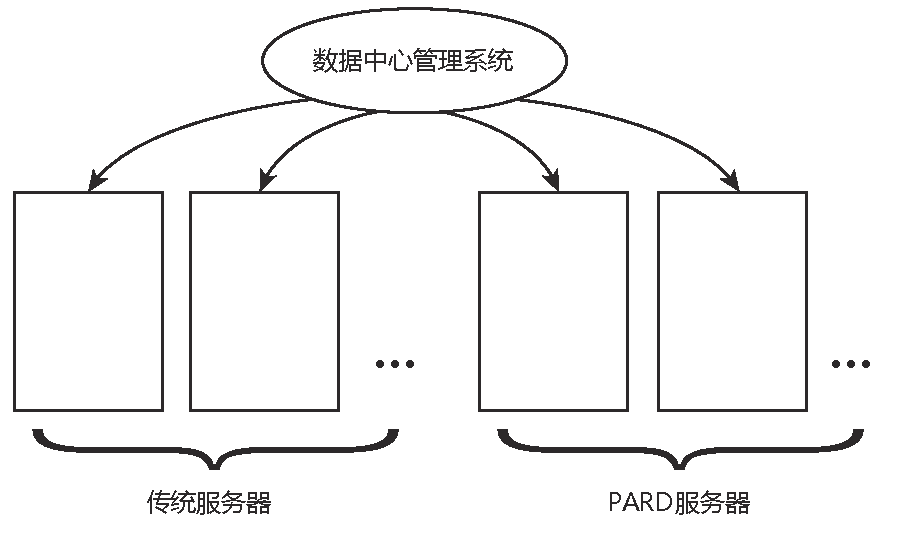
\includegraphics[width=0.6\textwidth]{swstk/pard-dc-overview}
  \caption{PARD服务器与数据中心管理系统}
  \label{fig:pard-dc-overview}
\end{figure}

\begin{table}[tb]
\begin{center}
\begin{tabular}{c|c|c}
  \toprule[1.5pt]
  & \textbf{Conventional Server} & \textbf{PARD Server}\\
  \midrule[1pt]
  \emph{Virtualization} & SW Supported & HW Supported\\
  \hline
  \emph{Perf. Isolation} & Unsupported & HW Surpported\\
  \hline
  \emph{Monitoring} & High overhead & Realtime\\
  \hline
  \emph{Perf. Adaption} & Coarse-grained  & Fine-grained\\
  \hline
%  \emph{Management} & Intergerited & Deccouple\\
%  \hline
  \bottomrule[1.5pt]
\end{tabular}
\caption{PARD服务器与传统服务器特性对比}
\label{tab:pard-features}
\end{center}
\end{table}

本章主要讨论如何将PARD服务器集成到现有数据中心管理系统,
并利用其提供的资源管理特性(表\ref{tab:pard-features})实现高效的数据中心管理。
未来数据中心传统服务器与PARD服务器共存,其架构如图\ref{fig:pard-dc-overview}所示,
两种类型的服务器由数据中心管理系统统一管理,为不同类型的应用提供服务。
PARD服务器与传统服务器主要的区别在于其提供了细粒度的资源管理、实时的性能监控、
硬件支持的虚拟化与性能隔离,因此更适合于短时多变的作业;
而长期运行,且负载稳定的应用可以通过软件管理的方式在传统服务器中运行。
为实现以上架构,需要考虑两个问题:
1)如何设计节点内资源管理,使其充分发挥PARD体系结构提供的硬件支持;
2)如何修改数据中心管理系统,使其能够支持PARD体系结构。
为解决以上两个问题,本节后续内容将对数据中心管理系统与节点内资源管理架构进行简要介绍。

%首先对数据中心管理系统进行简要介绍,
%然后对比已有节点内资源管理所需的软件栈支持,并
%带外管理相关内容。 介绍IPMI/BMC与带外管理,PARD的软件栈在此基础上进行扩充。


\subsection{数据中心管理系统}

\begin{figure}[tb]
  \centering
  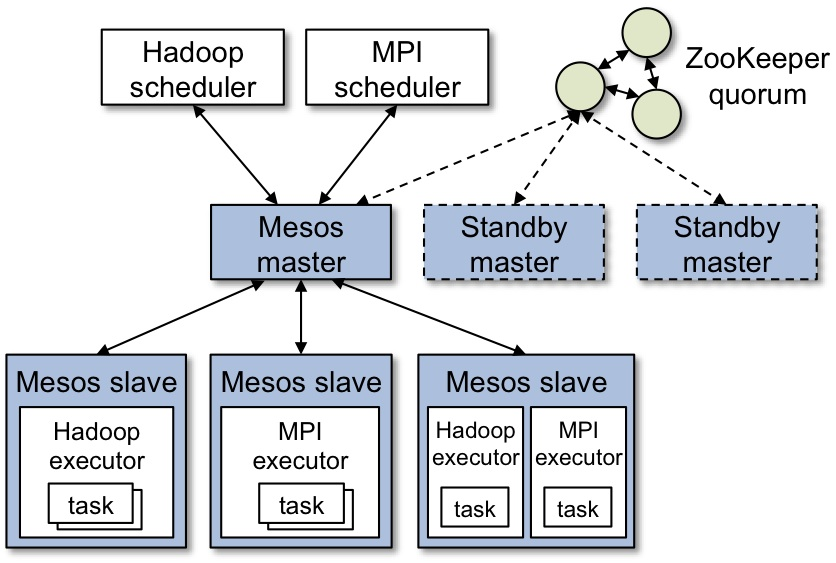
\includegraphics[width=0.7\textwidth]{swstk/mesos-arch}
  \caption{Mesos系统架构}
  \label{fig:mesos-arch}
\end{figure}

如上文所述,数据中心管理系统需要为数据中心提供高可用、高可靠、高利用率以及快速部署支持。
以Apache Mesos\cite{}为例,其架构如图\ref{fig:mesos-arch}所示,
它通过集中式的master节点控制运行在服务器内的slave守护进程实现数据中心资源管理。
master管理所有的资源,当slave注册到mesos集群时,将其提供的资源发送到master进行统一管理,
这些资源主要指CPU、内存、磁盘,除此之外还包括其他用户自定义类型的资源,
以资源列表的形式发送给master,如:

\textit{<slave ID, resource1:amount1, resource2:amount2, ...>}

mesos为用户提供framework抽象,主要包含两个部分:调度器(scheduler)与执行器(executor)。
其中调度器与master节点交互并获取资源,执行器在slave节点上运行,执行由调度器发送的任务(task)。
master根据用户设定的策略为每个framework分配资源,例如公平划分(fair sharing)或基于优先级的策略(strict priority)。
当master决定分配多少资源给framework后,它将资源列表发送到framework的调度器,
调度器从中选择其所需的资源,并将任务描述发送给master,由其分发到对应的slave节点执行。

%\textbf{mesos如何实现高可用、高可靠、高利用率以及快速部署?}
mesos只提供了最基本的资源管理与调度功能,
通过细粒度的资源管理与资源调度,实现了高利用率;
并提供基于进程或容器的快速应用部署。
通过自定义framework可以很容易的扩展mesos,
如Marathon\cite{}在mesos的基础上实现了应用自动扩容与出错重启,实现了高可用与高可靠。


\subsection{节点内资源管理架构}

数据中心管理系统所提供的功能需要节点内提供相应支持,包括资源分配与隔离、资源监控等。

有两种不同的架构实现节点内资源管理,一种是带内管理,另一种是带外管理。

带内管理是指:

带外管理是指:

上节介绍的mesos slave daemon相当于带内管理,其他数据中心管理系统基本上都是使用带内管理;
带内管理相比于带外管理最大的优点是,xxx。
但其缺点也很明显,xxx。

In computing, one form of out-of-band management is sometimes called lights-out management (or LOM) and involves the use of a dedicated management channel for device maintenance. It allows a system administrator to monitor and manage servers and other network-attached equipment by remote control regardless of whether the machine is powered on, or if an operating system is installed or functional.

By contrast, in-band management like VNC or SSH is based on in-band connectivity and software that must be installed on the remote system being managed and only works after the operating system has been booted. This solution may be cheaper, but in computing it does not allow access to firmware (BIOS or UEFI) settings, does not make it possible to reinstall the operating system remotely, and it cannot be used to fix problems that prevent the system from booting. In networking, it does not allow management of remote network components independently of the current status of other network components.

Both in-band and out-of-band (OOB) management are usually done through a network connection, but an out-of-band management card can use a physically separated network connector if preferred. A remote management card usually has at least partially independent power supply, and can power the main machine on and off through the network.


PARD体系结构采用带外管理的方式管理节点内的资源,其PRM的设计是源于服务器中IPMI/BMC的设计,并对其功能进行扩展。
原始的IPMI/BMC只提供了XXX的功能,其架构如图\ref{fig:ipmi-schem}所示,

The Intelligent Platform Management Interface (IPMI) is a set of computer interface specifications for an autonomous computer subsystem that provides management and monitoring capabilities independently of the host system's CPU, firmware (BIOS or UEFI) and operating system. IPMI defines a set of interfaces used by system administrators for out-of-band management of computer systems and monitoring of their operation. For example, IPMI provides a way to manage a computer that may be powered off or otherwise unresponsive by using a network connection to the hardware rather than to an operating system or login shell

\begin{figure}[tbh]
  \centering
  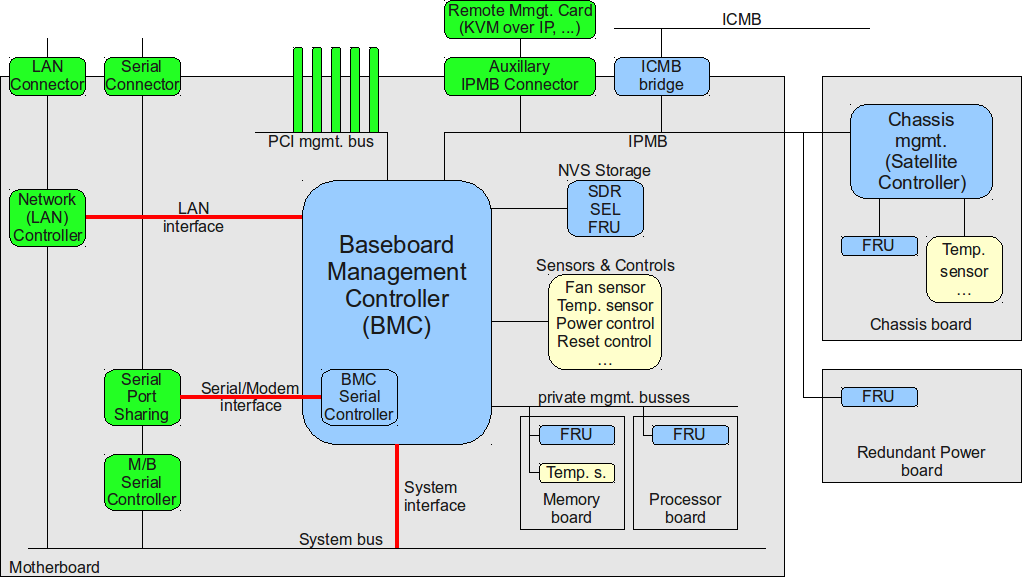
\includegraphics[width=0.95\textwidth]{swstk/ipmi-schem}
  \caption{IPMI结构框图}
  \label{fig:ipmi-schem}
\end{figure}

IPMI的结构如图\ref{fig:ipmi-schem}所示,其中主要包含以下几个模块:

\textbf{Baseboard Management Controller (BMC)}\quad
A micro-controller (BMC) is the heart of the IPMI architecture. The tasks of the BMC includes:
interfacing between the system management software and the hardware being used (through which the BMC has been connected using IPMB and ICMB)
monitoring independently
logging events independently
controlling recovery

\textbf{Intelligent Platform Management Bus (IPMB)}\quad
IPMI allows for the extension of the BMC by additional Management Controllers (MCs) through the application of the IPMB standard.
IPMB is an I²C based serial bus, which makes connection with various boards inside of one chassis possible. It is used for communication to and between the management controllers (MCs). Additional MCs are often designated Satellite Controllers.

\textbf{Intelligent Chassis Management Bus (ICMB)}\quad
ICMB provides a standardized interface for communication and control between chasses.

PRM在其基础上通过控制平面与控制平面网络,将资源管理功能也增加到其中,PRM具体架构在第\ref{chap:prm:arch}节将进行详细介绍。


\section{软件栈平台与架构}
\label{chap:prm:arch}

基于IPMI,增加控制平面网络,实现与控制平面通信

\begin{figure}[tbh]
  \centering
  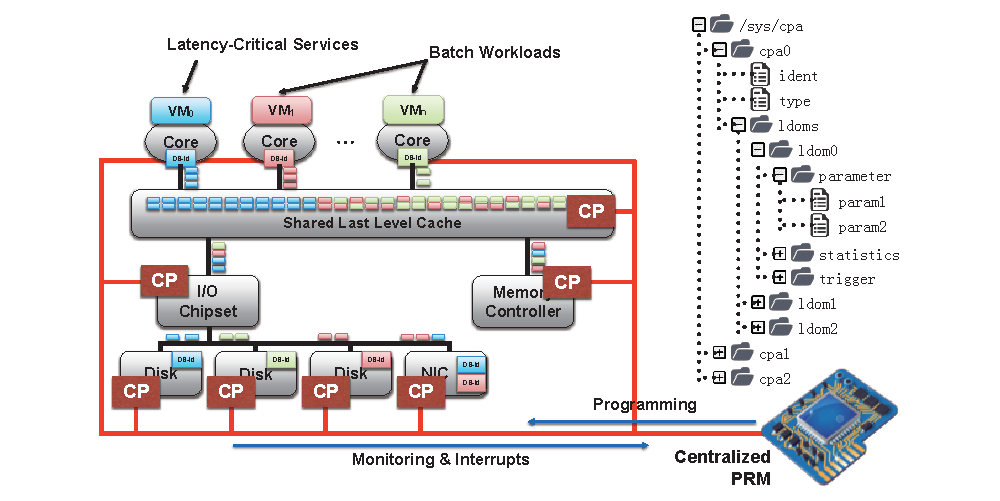
\includegraphics{arch/pard-arch-outline.pdf}
  \caption[PARD体系结构概况]{PARD体系结构概况}
  \label{fig:pard-arch-outline}
\end{figure}


Like IPMI [6] in conventional servers, PARD includes a
per-computer centralized platform resource manager (PRM) that
connects all control planes and tag registers (see the dash lines in
Figure 2). PRM is essentially an embedded system-on-chip (SoC)
that consists of an embedded processor, RAM, flash, a local bus, an
Ethernet adaptor and several control plane adaptors (CPAs).

A Linux-based firmware running on PRM abstracts all control
planes as a device file tree that is logically centralized. The
firmware provides a uniform file based programming interface to
access different control planes and a more advanced “trigger)action”
programming methodology (see below) for operators to create and
deploy resource management policies.


\section{节点内资源管理}

\subsection{控制平面抽象}

将控制平面抽象为文件,实现软件编程

To provide a uniform interface for firmware users (data center operators)
to access various control planes, we leverage Linux’s device
file mechanism. Figure 6 shows the abstraction of the control planes
from a firmware user’s perspective. Specifically, each control plane
is connected to a PRM’s control plane adaptor (CPA) that is abstracted
as a file and is mounted to the sysfs [55] of the firmware as
“/sys/cpa/cpa[0-9][0-9]*”. Thus firmware users can use either bash
commands (e.g., cat or echo) or system calls to access these files.
Each control plane file is organized as a subtree, which contains
some general information such as ident (e.g., cpa0’s “CACHE CP”
in Figure 6) and type indicating which type of a control plane
is, cache (“C”), memory (“M”) or I/O bridge (“B”). Besides, a
control plane file further includes several subtrees, each of which
represents a LDom with a specific DS-id. When a new LDom is
created, the firmware creates a new subtree with root “ldom[0-9][0-
9]*” under the node ldoms, where the number represent a DS-id.
Take the ldom0 subtree as an example, there are three tiny trees
with roots as parameters, statistics and triggers respectively, which
are mapped to several rows of the three tables of the LLC control
plane.

Programming Methodology
As mentioned in x3, we adopt a “trigger)action” programming
methodology. Data center operators predefine a set of trigger)action
rules for different priorities. Usually a trigger is based on performance
metrics, e.g., “MissRate>30%”.
Example 1 in Figure 6 demonstrates how to install a trigger)action
rule. A data center operator uses the pardtrigger command to program
the trigger condition “MissRate>30%” for “ldom=0” (i.e.,
DS-id=0) into the trigger table of the cache control plane (cpa0).
The parameter “action=0” guides the command to create a leaf
node “0” under “.../cpa0/ldoms/ldom0/triggers”. Then the operator
calls “echo ...” to install the action script “/cpa0 ldom0 t0.sh”
shown in Example 2.
There are two programming approaches based on the device file
tree. One is invoking system calls (open/read/write etc.) to open
and manipulate a CPA file. For example, the pardtrigger command
is written in C and invokes syscalls to install a trigger into the
cache control plane. The advantage of this approach is very fast. A
more convenient approach is leveraging bash commands to directly
access these CPA files, as shown in Example 2.


\subsection{实现虚拟机}


\subsection{实现QoS管理}


\section{与数据中心结合}

% 云计算三种模型
云计算有三种模式:SaaS、PaaS、IaaS,如图\ref{fig:cloud-usage-model}所示,
其区别在于用户需要管理的层次
其中IaaS用户需要管理到OS层,以OpenStack为例;
PaaS用户只需要管理应用与数据,其他部分由数据中心管理,以Docker为例;
SaaS是最底层,用户直接使用不同软件组合,以XX为例。
本章主要考查IaaS与PaaS两种模式。

\begin{figure}[tb]
  \centering
  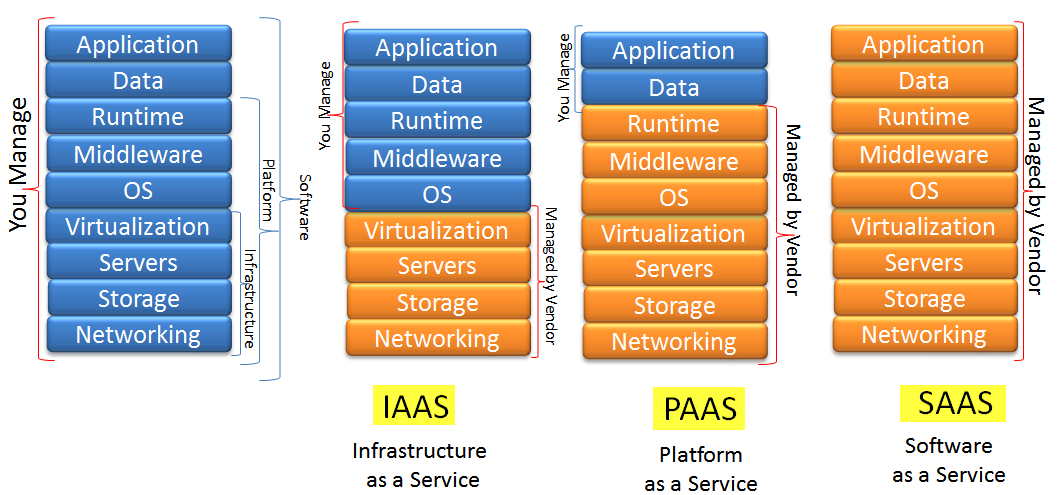
\includegraphics[width=0.8\textwidth]{swstk/cloud-usage-model}
  \caption{云计算3种使用模式对比:IaaS、PaaS与SaaS}
  \label{fig:cloud-usage-model}
\end{figure}

PARD提供的逻辑域抽象,能够很容易的实现IaaS模式,
因为逻辑域抽象与虚拟机抽象几乎完全类似,之前几章的工作都是基于IaaS模式对PARD进行讨论,
但目前数据中心PaaS由于资源浪费较少,被越来越广泛的使用,
本节主要讨论如何在PARD平台上实现PaaS模式,同时将其集成到数据中心管理系统中,
这里将主要针对mesos系统进行讨论。

\subsection{使用PARD体系结构实现PaaS}
% PARD如何实现PaaS
PARD实现PaaS的方式是通过类似于unikernel/LibOS的方式,
用户提供应用,PARD软件栈提供OS kernel,并将两者组合运行在逻辑域中。
具体流程如下,如图\ref{fig:pard-ldom-paas}:

1)用户提供需要执行的应用与数据,并选择所需的运行时环境和库;

2)将应用、数据、运行时环境打包为一个package,完成应用构建阶段;

3)系统根据用户选择的硬件资源配置创建逻辑域,将选择的内核与打包好的应用一起加载到逻辑域中;

4)将逻辑域在PARD服务器上启动。

\begin{figure}[tb]
  \centering
  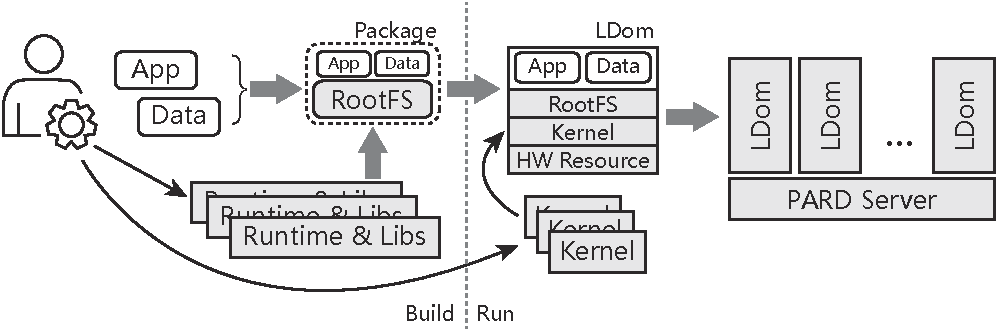
\includegraphics[width=\textwidth]{swstk/pard-ldom-paas}
  \caption{PARD体系结构实现PaaS模式}
  \label{fig:pard-ldom-paas}
\end{figure}

通过以上方式实现硬件支持的容器,该方法也可以在其它只提供IaaS抽象的场景中实现PaaS的功能。

\subsection{mesos系统集成}
% mesos如何管理资源

% PARD如何支持MesosExecutor


\subsection{PARD体系结构对数据中心管理系统的影响}
% 对mesos资源模型的影响
%  -- PARD为mesos增加了额外可控制的资源
%  -- mesos如何管理这些额外的资源
%    -- 增加资源抽象属性:CPU/Mem => Cache/BW/QoS-Level/etc.
%    -- 增加调度考查

\section{小结}


应用负载具有波动性,对硬件资源的需求会发生变化,需要提供一种动态调整应用资源分配的方案。

有三个层次,分别:
(1)节点内不同硬件资源的协同管理;
(2)节点内应用调度与资源协同管理;
(3)节点间协同管理;


PRM软件接口,

- 与mesos集成,实现硬件支持的容器

- 与OpenStack集成,实现IaaS平台

- 与SDN集成,实现网络中心的系统

